\section{Theory} \label{sec:theory}
% Physics part
% - Composition (photometry) -> telescope optics?/instrument?/bit depth?
% - Trajectories and relative trajectory of spacecraft, especially trajectories for flybys
% - Star rendering?
% - Describe physics of SSSBs, i.e. size/shapes/surface (features/color/albedo) illumination
%
% Computer Science part
% - Physics-based rendering? -Shaders/procedural terrain generation
% - Compression
% - Reconstruction (SfM), relates to camera physics. Generally Computer Vision topic.
% - Image processing Gaussian filtering, downscale local means
% - Logic for choosing number of reconstructed points as quality measure
%
% Space
% - Small Spacecrafts -> small data budgets?
%
% Max Science?
% Navigation/autonomy?
%
% Concepts to describe???

\subsection{Small Solar System Body}
The \gls{iau} defines a \gls{sssb} as any object in the Solar System, that is not a planet, dwarf planet or satellite \cite{iau_sssb}. Therefore, most asteroids, comets, Trans-Neptunian Objects, minor planets, meteorites and interplanetary dust are included in this definition \cite{wiki:sssb}. This is visualised in Figure \ref{fig:sssb_diagram}. Within this work, the term \gls{sssb} refers to asteroids and comets.

\begin{figure}[htb]
    \centering
    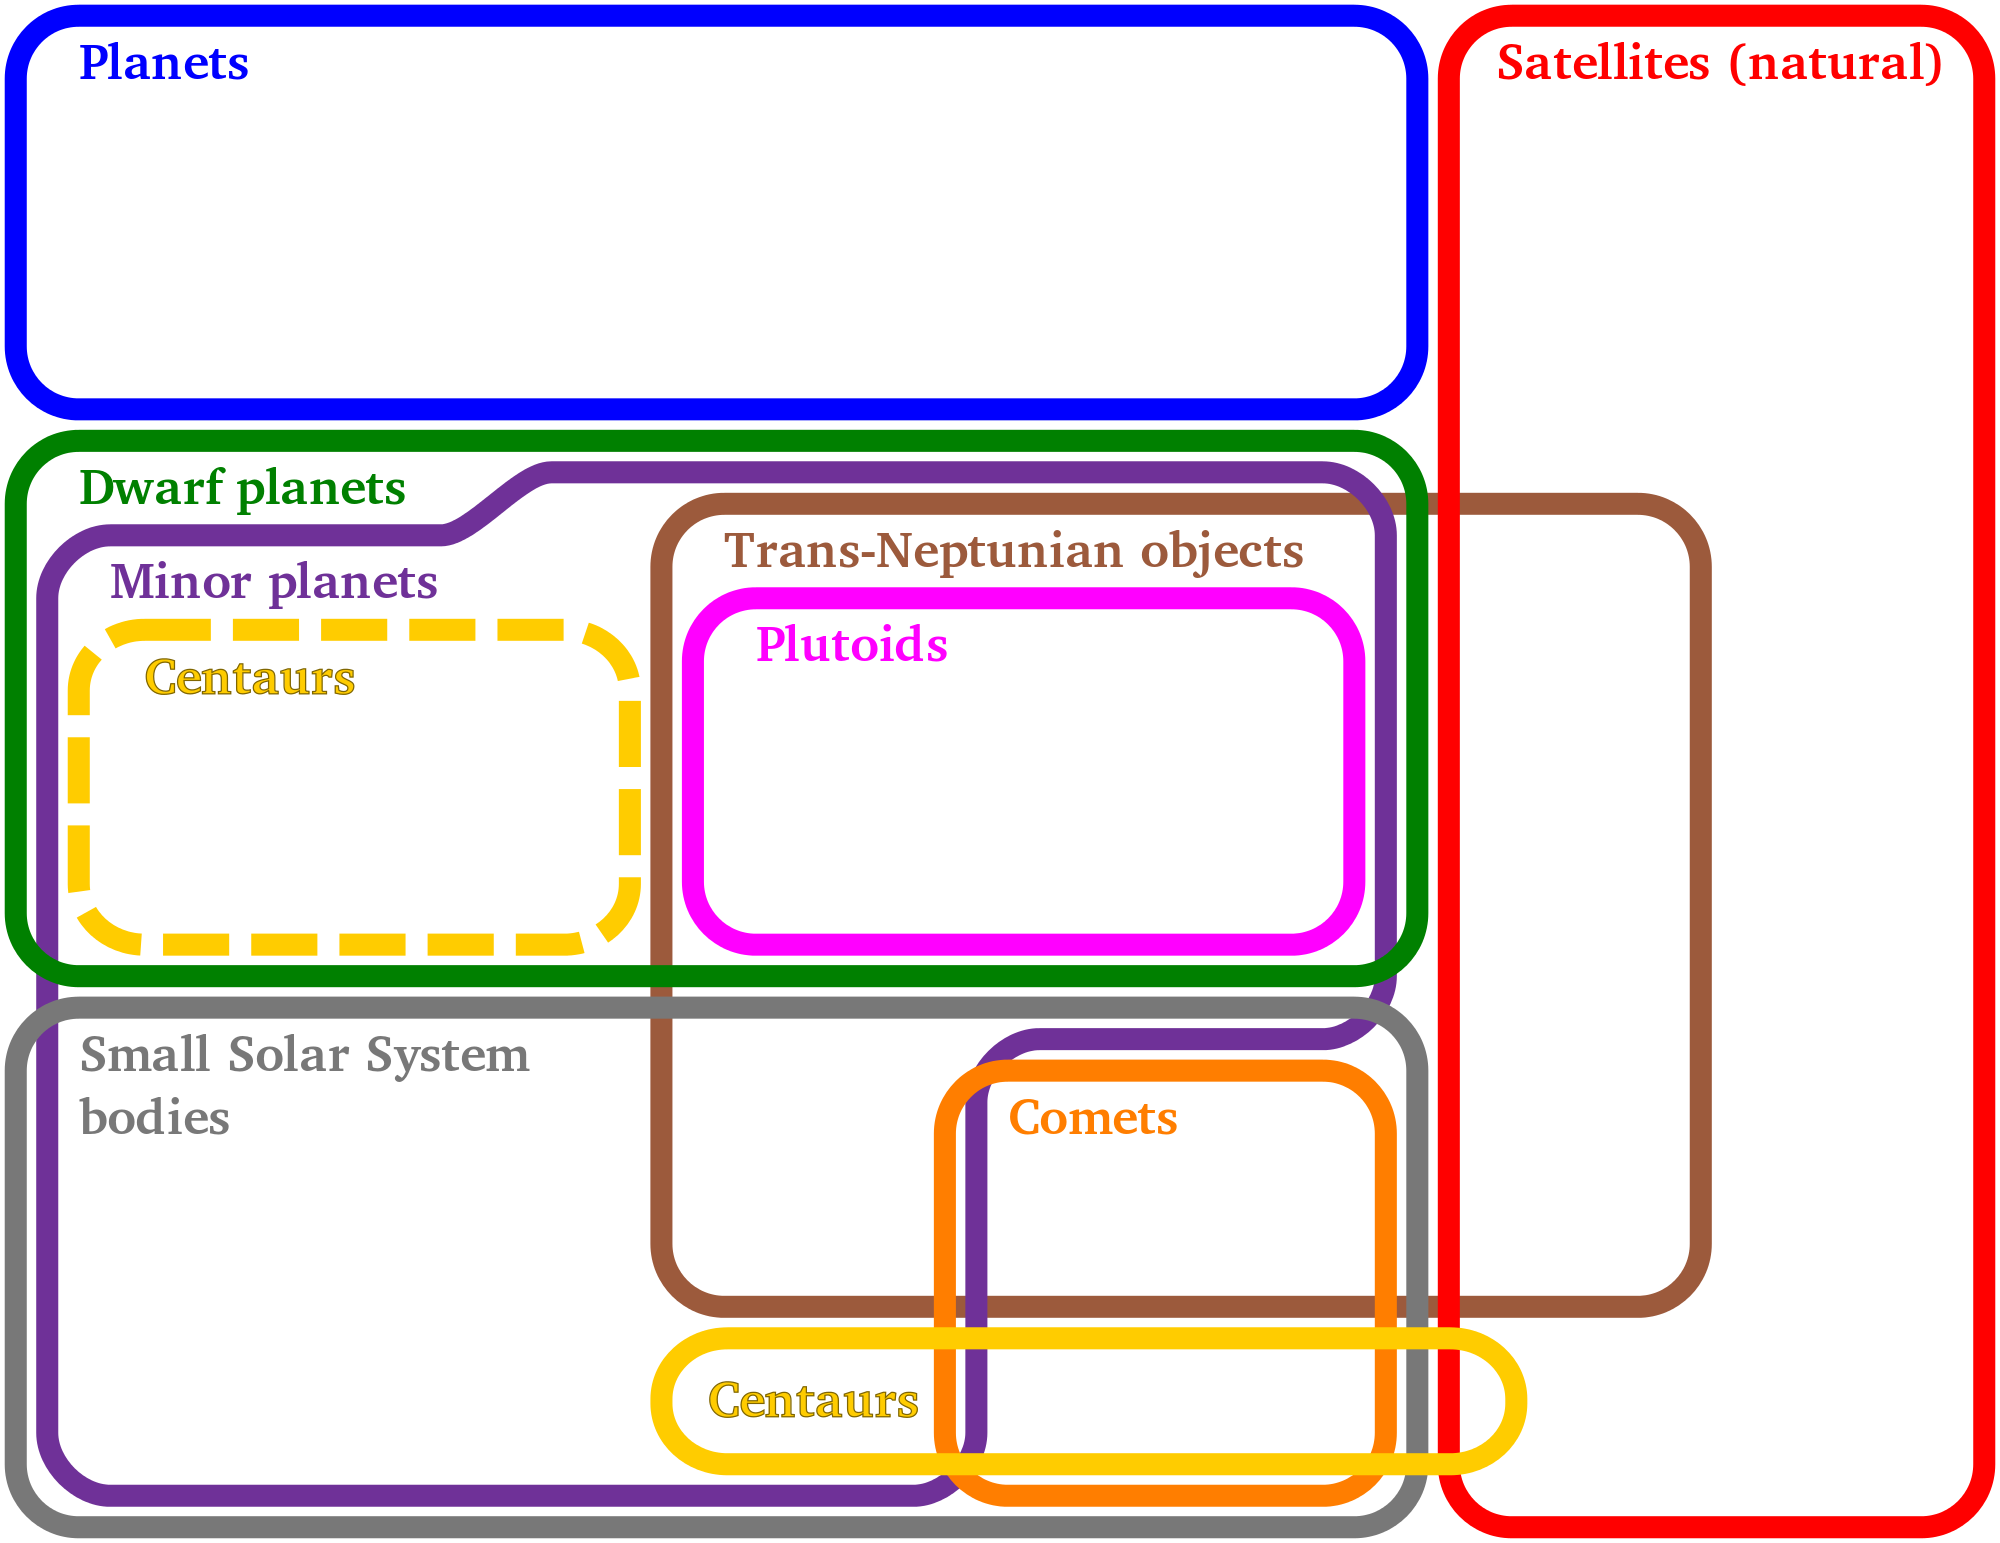
\includegraphics[width=\textwidth]{doc/thesis/0_figures/Euler_diagram_of_solar_system_bodies.png}
    \caption{Diagram of which types of bodies the \gls{sssb} definition includes \cite{wiki:sssb}.}
    \label{fig:sssb_diagram}
\end{figure}

\subsection{Asteroids}

\subsection{Comets}